\documentclass[10pt,a4paper]{article}

\usepackage[utf8]{inputenc}
\usepackage[a4paper,margin=22mm,top=20mm,bottom=22mm]{geometry}
\usepackage{microtype}
\usepackage{parskip}
\usepackage{booktabs}
\usepackage{tabularx}
\usepackage{array}
\usepackage{enumitem}
\usepackage{titlesec}
\usepackage{xcolor}
\usepackage{caption}
\usepackage{graphicx}
\usepackage{tikz}
\usetikzlibrary{arrows.meta,patterns,positioning}
\usepackage[hidelinks]{hyperref}

\definecolor{accent}{HTML}{1F4E79}
\definecolor{rulegray}{HTML}{B8BEC6}
\definecolor{done}{HTML}{2E7D32}
\definecolor{wip}{HTML}{B26A00}
\definecolor{todo}{HTML}{6B7280}

\titleformat{\section}{\large\bfseries\color{accent}}{\thesection}{0.6em}{}
\titlespacing*{\section}{0pt}{1.4em}{0.5em}
\setlist{nosep,leftmargin=1.4em}
\renewcommand{\arraystretch}{1.25}
\captionsetup{font=small,labelfont=bf}
\newcolumntype{L}{>{\raggedright\arraybackslash}X}
\newcommand{\code}[1]{\texttt{#1}}
\newcommand{\sdone}{\textcolor{done}{\textbf{done}}}
\newcommand{\swip}{\textcolor{wip}{\textbf{started}}}
\newcommand{\stodo}{\textcolor{todo}{not started}}

\begin{document}

{\LARGE\bfseries\color{accent} Mechanics Sketch Tool}\\[0.3em]
{\large Status report and build plan}\hfill{\large 9 October 2026}\\[-0.4em]
{\color{rulegray}\rule{\textwidth}{0.6pt}}

\section{Summary}

The sketcher works: steps 1 to 5 of the build plan are done. Geometry can be
drawn, constrained, dimensioned and dragged, and editing a dimension
re-solves the whole drawing. It runs as a single HTML file that opens
straight from disk. Supports, loads, the TikZ and SVG exports and the
desktop install are still to come (steps 6 to 8).

The tool is a CAD-style constraint sketcher for truss and beam figures:
geometry is drawn freely, constrained and dimensioned afterwards, and figures
will export to both TikZ and SVG for use in \LaTeX.

\begin{figure}[h]
\centering
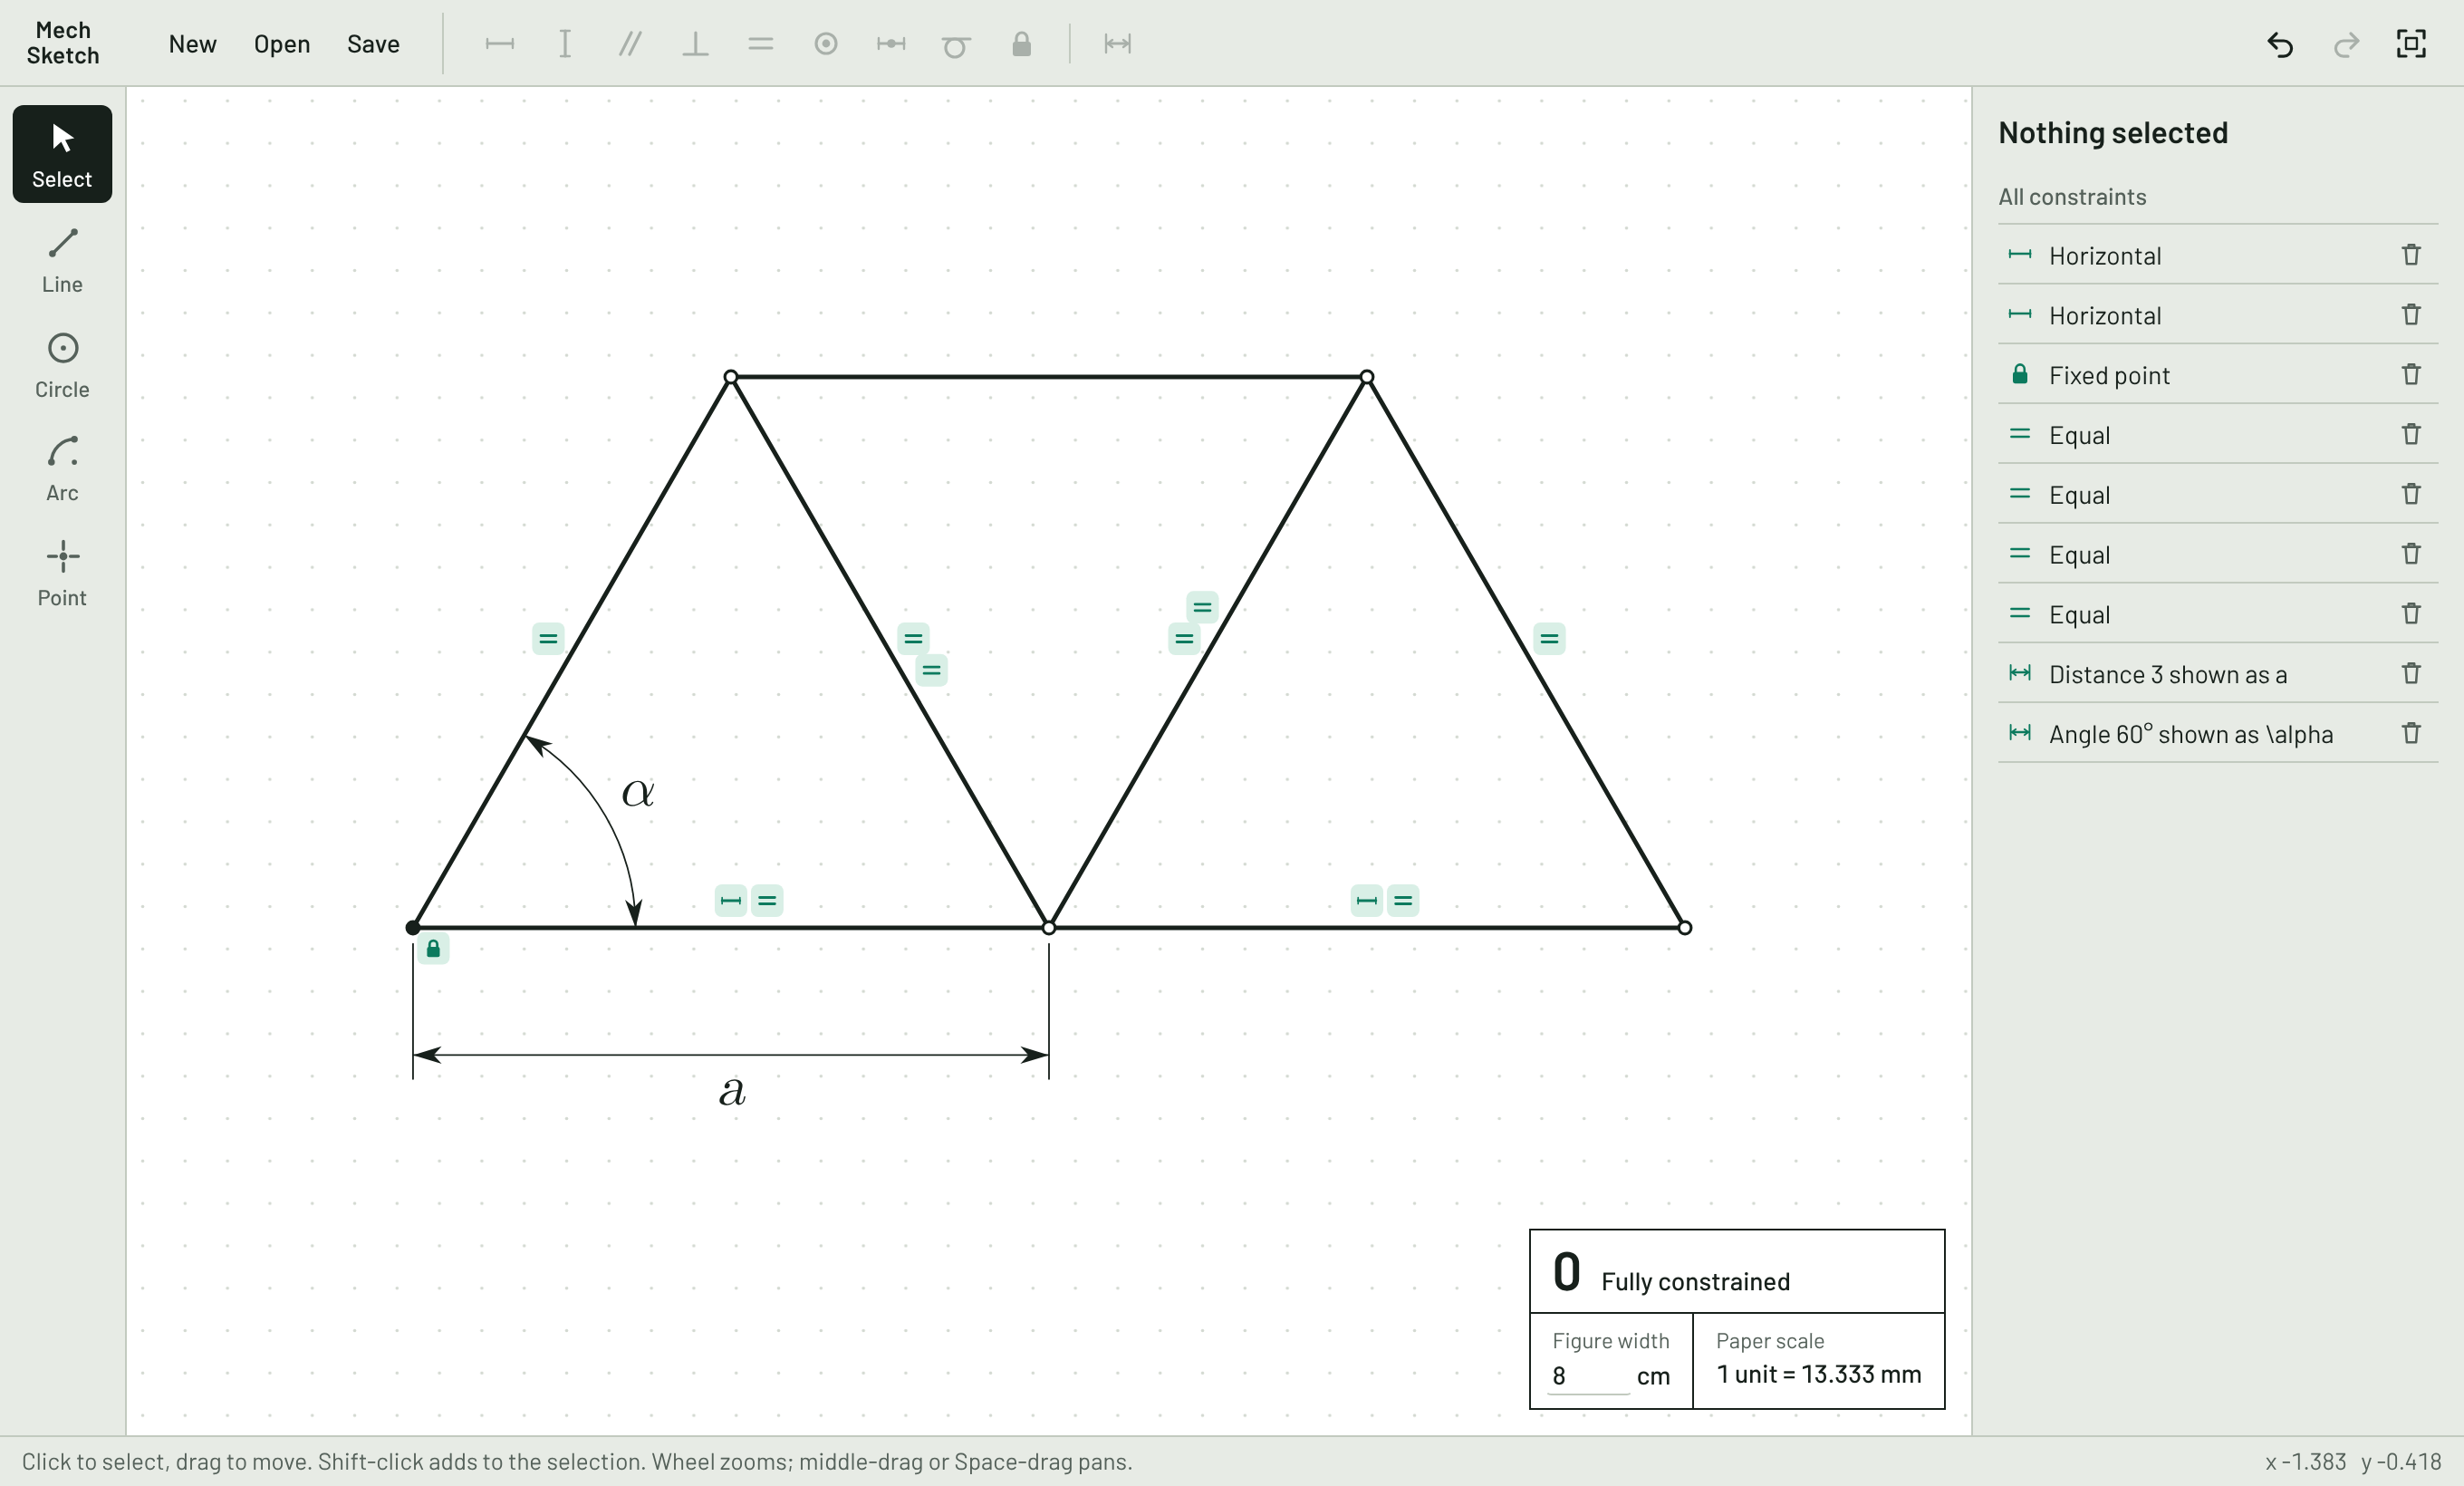
\includegraphics[width=\textwidth]{screenshot.png}
\caption{The current build with a Warren truss. One fixed joint, two
horizontal chords, equal-length members, one length $a$ and one angle
$\alpha$ leave zero degrees of freedom.}
\end{figure}

\section{Decisions}

\begin{tabularx}{\textwidth}{@{}>{\bfseries}p{28mm}L@{}}
\toprule
Platform & Browser app, installable as a PWA: one click gives a desktop icon, its own window and offline use. \\
Stack & TypeScript and Vite. The canvas is drawn directly in SVG. \\
Solver & FreeCAD's 2D solver \code{planegcs}, used through its WebAssembly build (\code{@salusoft89/planegcs} 1.3.0, LGPL). Not written from scratch. \\
Exports & TikZ and SVG, both first-class, generated from one shared primitive list. \\
Labels & Typed as \LaTeX{} strings (\code{F\_1}, \code{\textbackslash alpha}) and previewed with MathJax. \\
Hosting & GitHub Pages, needed for the PWA install. The repository does not exist yet (Section~\ref{sec:open}). \\
\bottomrule
\end{tabularx}

\section{Feature scope for the first version}

\begin{tabularx}{\textwidth}{@{}>{\bfseries}p{28mm}L@{}}
\toprule
Geometry & Points, lines, circles, arcs. \\
Constraints & Coincident, horizontal, vertical, parallel, perpendicular, equal length, fixed point. \\
Dimensions & Distance, angle, radius. Each holds a driving value for the solver and a separate display label such as $2a$, and can be hidden. \\
Supports & Pin, roller and fixed support, with ground hatching. \\
Loads & Force arrows, moments, distributed loads. \\
Editing & Snapping, auto-constraints while drawing (near-horizontal becomes horizontal), dragging of under-constrained geometry, undo and redo. \\
Feedback & Remaining degrees of freedom; conflicting and redundant constraints are flagged. \\
Files & Save and load as JSON, SVG export, TikZ export with a ``Copy TikZ'' button. \\
\bottomrule
\end{tabularx}

Built so far: geometry, constraints, dimensions, editing, feedback, and
save and load. Supports, loads and the two exports are not built yet.

\textbf{Added beyond the agreed list,} because the solver provides them
directly: point on a line or circle, midpoint, tangent, equal radius, and
construction geometry (dashed in the editor, left out of exports).

\textbf{Out of scope:} springs, dampers, masses, velocity and angular
velocity arrows, coordinate frames.

\section{Direction}

\begin{figure}[h]
\centering
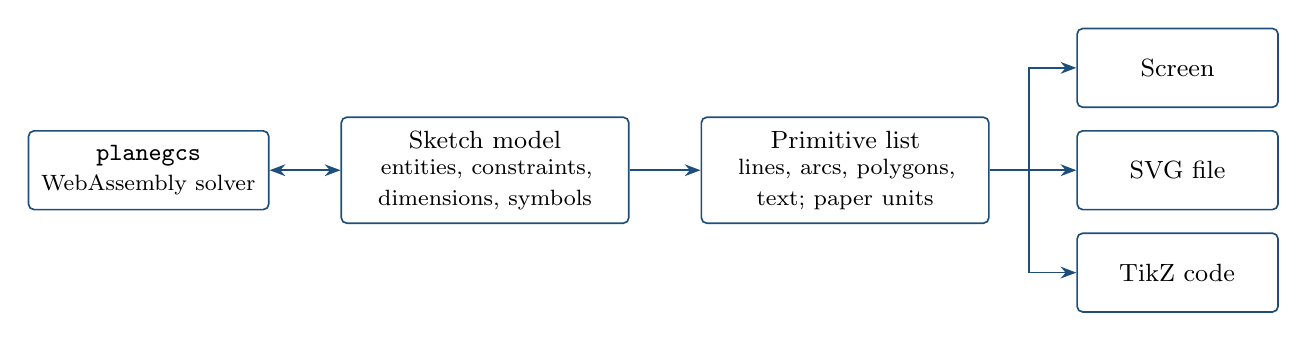
\begin{tikzpicture}[
  box/.style={draw=accent, line width=0.6pt, rounded corners=2pt, align=center,
              inner sep=5pt, font=\small, minimum height=10mm},
  flow/.style={-{Stealth[length=2mm]}, line width=0.6pt, color=accent},
  both/.style={{Stealth[length=2mm]}-{Stealth[length=2mm]}, line width=0.6pt, color=accent}]
  \node[box, text width=33mm] (model) {Sketch model\\{\footnotesize entities, constraints,\\dimensions, symbols}};
  \node[box, text width=27mm, left=9mm of model] (solver) {\code{planegcs}\\{\footnotesize WebAssembly solver}};
  \node[box, text width=33mm, right=9mm of model] (prims) {Primitive list\\{\footnotesize lines, arcs, polygons,\\text; paper units}};
  \node[box, text width=22mm, right=11mm of prims, yshift=13mm] (screen) {Screen};
  \node[box, text width=22mm, right=11mm of prims] (svg) {SVG file};
  \node[box, text width=22mm, right=11mm of prims, yshift=-13mm] (tikz) {TikZ code};
  \draw[both] (solver) -- (model);
  \draw[flow] (model) -- (prims);
  \draw[flow] (prims.east) -- ++(5mm,0) |- (screen.west);
  \draw[flow] (prims.east) -- (svg.west);
  \draw[flow] (prims.east) -- ++(5mm,0) |- (tikz.west);
\end{tikzpicture}
\caption{Data flow. Every edit goes through the solver; all three outputs
are drawn from the same primitive list.}
\end{figure}

Four rules shape the code:

\begin{enumerate}
\item \textbf{One primitive list feeds every output.} Supports, hatching,
arrows and dimensions are broken down into lines, arcs, polygons and text
once. The screen, the SVG writer and the TikZ writer all read that list, so
the exports cannot drift away from what is on screen.
\item \textbf{Symbols are sized in paper units.} A pin support is the same
few millimetres wide whether the truss is 3\,m or 300\,mm long. The same
holds for arrowheads, line widths and text.
\item \textbf{The figure has a set width.} With the width fixed (8\,cm, for
example), the editor shows labels at their true size relative to the
geometry, so anything that does not collide on screen will not collide in
the PDF.
\item \textbf{Symbols stay out of the solver.} Supports and loads are
attached to points and lines and follow them. Only geometry, constraints
and dimensions are solved.
\end{enumerate}

\begin{figure}[h]
\centering
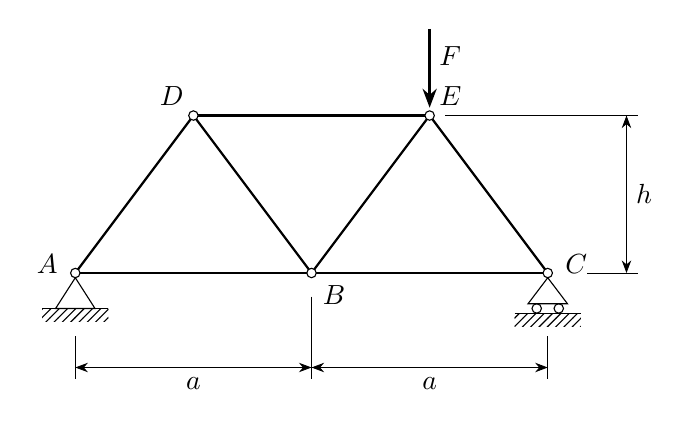
\begin{tikzpicture}[
  member/.style={line width=0.8pt, line cap=round, line join=round},
  thin/.style={line width=0.4pt},
  dim/.style={{Stealth[length=1.6mm]}-{Stealth[length=1.6mm]}, line width=0.3pt},
  ext/.style={line width=0.3pt},
  force/.style={-{Stealth[length=2.4mm]}, line width=0.9pt}]
  % members
  \draw[member] (0,0) -- (3,0) -- (6,0);
  \draw[member] (0,0) -- (1.5,2) -- (3,0) -- (4.5,2) -- (6,0);
  \draw[member] (1.5,2) -- (4.5,2);
  \foreach \p in {(0,0),(3,0),(6,0),(1.5,2),(4.5,2)} \fill[white, draw=black, thin] \p circle (0.06);
  % pin support at A
  \draw[thin, fill=white] (0,-0.06) -- (-0.25,-0.45) -- (0.25,-0.45) -- cycle;
  \fill[pattern=north east lines] (-0.42,-0.62) rectangle (0.42,-0.45);
  \draw[thin] (-0.42,-0.45) -- (0.42,-0.45);
  % roller support at C
  \draw[thin, fill=white] (6,-0.06) -- (5.75,-0.39) -- (6.25,-0.39) -- cycle;
  \draw[thin] (5.86,-0.45) circle (0.06) (6.14,-0.45) circle (0.06);
  \fill[pattern=north east lines] (5.58,-0.68) rectangle (6.42,-0.51);
  \draw[thin] (5.58,-0.51) -- (6.42,-0.51);
  % load
  \draw[force] (4.5,3.1) -- (4.5,2.1);
  \node[right] at (4.5,2.75) {$F$};
  % labels
  \node[left] at (-0.1,0.12) {$A$};
  \node[below right] at (3.02,-0.04) {$B$};
  \node[right] at (6.1,0.12) {$C$};
  \node[above left] at (1.5,2) {$D$};
  \node[above right] at (4.5,2) {$E$};
  % dimensions
  \draw[ext] (0,-0.8) -- (0,-1.35) (3,-0.3) -- (3,-1.35) (6,-0.8) -- (6,-1.35);
  \draw[dim] (0,-1.2) -- node[below] {$a$} (3,-1.2);
  \draw[dim] (3,-1.2) -- node[below] {$a$} (6,-1.2);
  \draw[ext] (6.5,0) -- (7.15,0) (4.7,2) -- (7.15,2);
  \draw[dim] (7,0) -- node[right] {$h$} (7,2);
\end{tikzpicture}
\caption{The kind of figure the tool should produce. This one is written
by hand; the labels are typeset by \LaTeX{}, so they match the document
font.}
\end{figure}

\section{Build plan}

\begin{tabularx}{\textwidth}{@{}c>{\bfseries\raggedright\arraybackslash}p{31mm}Lp{17mm}@{}}
\toprule
& Step & Contents & Status \\
\midrule
1 & Scaffold and data model & Project setup; types for entities, constraints and dimensions; JSON save and load; undo stack. Symbol types come with step 6. & \sdone \\
2 & Solver bridge & Translate the model to \code{planegcs} and back. Tested without a user interface on a known truss. & \sdone \\
3 & Canvas and drawing tools & Pan and zoom; point, line, circle and arc tools; snapping; auto-constraints; select and delete. & \sdone \\
4 & Constraints and dragging & Constraint toolbar; dragging through the solver; feedback on conflicts and degrees of freedom. & \sdone \\
5 & Dimensions & Place, edit the value by double-click, set the label, hide or show. & \sdone \\
6 & Symbols and labels & Supports, hatching, loads, MathJax labels, figure width setting. & \stodo \\
7 & Exports & SVG and TikZ writers. The TikZ output is compiled with \LaTeX{} and compared against the SVG. & \stodo \\
8 & PWA and polish & Install manifest, offline support, icon, keyboard shortcuts, deployment to GitHub Pages. & \stodo \\
\bottomrule
\end{tabularx}

This build covers steps 1 to 5. The next runnable builds follow step 7
(exports working) and step 8 (installable).

\section{What has been checked}\label{sec:verified}

\begin{itemize}
\item \textbf{Automated tests: 33 pass.} They cover the solver bridge (every
constraint and dimension type, dragging, conflict and redundancy reports),
the model (delete clean-up, JSON round trip), the primitive list (dimension
layout, paper scale, picking) and the label preview.
\item \textbf{Re-solve on a dimension change.} An isosceles truss triangle
with base 4 and height 3 solved to joints at $(0,0)$, $(4,0)$, $(2,3)$;
changing the values to 6 and 2 gave $(0,0)$, $(6,0)$, $(3,2)$.
\item \textbf{The app, driven in a browser.} Drawing with snapping, the
Warren truss in Figure~1 built from scratch through the interface
(the angle of $60^\circ$ put the top chord at $3\sin 60^\circ = 2.598$ above
the bottom one, as it should), dragging, undo and redo, box selection,
delete, save and open, reload restoring the last sketch, and rejecting a
conflicting constraint and an over-constraining dimension with a message.
\item \textbf{The single-file build.} Opened from disk with no server; it
drew, dimensioned and restored its sketch after a reload.
\item \textbf{Speed.} A truss with 77 members (117 entities) re-solves in about 4\,ms
per drag step.
\end{itemize}

Not checked: browsers other than Chromium, and touch input.

\section{Known limits of this build}

\begin{itemize}
\item \textbf{Colour is all or nothing.} Geometry is blue while the sketch has
any freedom left and black once it has none. The solver build does not report
which individual joints are still free.
\item \textbf{Label preview is a stand-in.} Labels such as \code{F\_1},
\code{2a} and \code{\textbackslash alpha} show with sub- and superscripts and
Greek letters in a serif font. MathJax replaces this in step 6. The TikZ
export will pass labels to \LaTeX{} unchanged either way.
\item \textbf{Figure width means geometry width.} Dimensions drawn outside the
geometry add to the final width.
\item \textbf{An unanchored sketch drifts.} Dragging one joint can shift the
others until a point is fixed.
\end{itemize}

\section{Open items}\label{sec:open}

\begin{itemize}
\item \textbf{Repository.} The connected GitHub account has one repository,
which belongs to a different project. The tool needs its own, and I cannot
create repositories from here. The code is committed locally and ready to
push. The desktop shortcut (step 8) depends on the repository, because the
install needs the app served over HTTPS.
\item \textbf{Solver licence.} \code{planegcs} is LGPL. That is fine for a
personal tool and for a public repository, provided the licence notice is
kept; the README carries it.
\item \textbf{Name.} ``Mech Sketch'' is a working title.
\end{itemize}

\end{document}
